\chapter{Implementación}\label{cap4}

\section{Tecnologías utilizadas}
\subsection{Base de datos relacional}\label{sec-bd-r}
Una base de datos relaciones es una colección de tablas relacionadas entre sí. La colección de tablas se describe a sí misma en cuanto a que el significado de los datos contenidos pertenecen a un mismo ámbito\cite{DataBaseConcepts}.\\
Una base de datos es administrada mediante un Sistema Administrador de Bases de Datos (DBMS por sus siglas en inglés), un DBMS es un programa de computadora usado para crear, procesas y administrar bases de datos. El DBMS recibe peticiones en lenguaje SQL (como se describe más adelante) y traduce esas peticiones a acciones dentro de la base de datos\cite{DataBaseConcepts}.\\
Para el desarrollo del proyecto AutoSA se han ocupado los siguientes conceptos:
\begin{enumerate}
	\item \textbf{Tabla}: una tabla es un conjunto de renglones (registros) y columnas (atributos) que cumple con las siguientes características\cite{DataBaseConcepts}:
	\begin{enumerate}
		\item Los renglones contienen unicamente datos relacionados con la tabla.
		\item Las entradas de una columna contienen un solo valor.
		\item Todas las entradas de una columna son del mismo tipo.
		\item Las columnas tienen un nombre único dentro de la tabla.
		\item El orden de las columnas y los renglones no es relevante.
		\item No contiene dos renglones idénticos.
	\end{enumerate}
	\item \textbf{Vista}: es una tabla derivada de una consulta de otras tablas, estas tablas pueden ser tablas de la base de datos o vistas definidas previamente. Una vista es considerada como tabla virtual porque no necesariamente existe físicamente a diferencia de una tabla de la base cuyas tuplas siempre están almacenadas físicamente en la base de datos\cite{FundamentalsOfDBSystems}.
	\item \textbf{Llave primaria}: es el conjunto de columnas que identifican de manera unívoca a cada renglón de la tabla.\cite{DataBaseConcepts}
	\item \textbf{Llave foránea}: define la relación de una tabla, \textbf{A}, hacia otra \textbf{B} y satisface las siguientes condiciones\cite{FundamentalsOfDBSystems, DataBaseConcepts}:
	\begin{enumerate}
		\item Los atributos de las tablas \textbf{A} y \textbf{B} son del mismo tipo y se corresponden uno a uno.
		\item Los atributos en la tabla \textbf{B} son exactamente los mismos de la llave primaria de la tabla \textbf{B}.
	\end{enumerate}
	\item \textbf{Restricción $NOT$ $NULL$}: indica que el valor del atributo no puede ser nulo\cite{FundamentosSistemasBasesDatos}. 
	\item \textbf{Índice}: es una estructura auxiliar para agilizar la obtención de registros. Los índices proveen rutas de acceso alternativo a los registros de la base de datos sin afectar la colocación física de los registros\cite{FundamentalsOfDBSystems}.
	\item \textbf{Lenguaje Estructurado de Consulta}\label{sec-sql}: del inglés Structured Query Language (SQL), fue desarrollado por IBM\textsuperscript{\textcopyright} al final de los años 70, es un lenguaje de datos orientado a texto, ha sido avalado por el Instituto Nacional de Estándares Americanos (ANSI por sus siglas en inglés) dando así los estándares ANSI para SQL, principalmente para este trabajo el estándar ANSI-92 o SQL-92.
	\item \textbf{Lenguaje de Definición de Datos}: DDL por sus siglas en inglés, es un lenguaje de SQL cuya función es describir la creación de estructuras tales como tablas, índices y restricciones, entre otras\cite{DataBaseConcepts}.
	\item \textbf{Lenguaje de Modelado de Datos}: DML por sus siglas en inglés, es un lenguaje de SQL cuya función es describir la modificación de datos, es decir, sentencias de inserción, borrado y actualización de datos\cite{DataBaseConcepts}.  
\end{enumerate}

\iffalse
\subsection{Java}\label{sec-java}

\begin{quote}
	Java is related to C++, which is a direct descendant of C. Much of the character of Java is inherited from these two languages. From C, Java derives its syntax. Many of Java’s objectoriented features were influenced by C++. In fact, several of Java’s defining characteristics come from—or are responses to—its predecessors. Moreover, the creation of Java was deeply rooted in the process of refinement and adaptation that has been occurring in computer programming languages for the past several decades. For these reasons, this section reviews the sequence of events and forces that led to Java. As you will see, each innovation in language design was driven by the need to solve a fundamental problem that the preceding languages could not solve. Java is no exception\cite{JavaCompleteReference}.
\end{quote}

\begin{quote}
	Java was conceived by James Gosling, Patrick Naughton, Chris Warth, Ed Frank, and Mike Sheridan at Sun Microsystems, Inc. in 1991. It took 18 months to develop the first working version. This language was initially called “Oak,” but was renamed “Java” in 1995. Between the initial implementation of Oak in the fall of 1992 and the public announcement of Java in the spring of 1995, many more people contributed to the design and evolution of the language. Bill Joy, Arthur van Hoff, Jonathan Payne, Frank Yellin, and Tim Lindholm were key contributors to the maturing of the original prototype\cite{JavaCompleteReference}.
\end{quote}

Java es un lenguaje bonito porque gracias a él  puedo obtener dinero para hacer las cosas que me gustan como comer  y jugar squash

\subsection{Javascript}\label{sec-javascript}
\fi


\subsection{Sahi}\label{sec-sahi}
La compañía Sahi Pro\textsuperscript{\textcopyright}\cite{SahiPro} describe a su producto del mismo nombre como:
\begin{quote}
	Sahi es una herramienta enfocada a la automatización de pruebas para servicios Web, plataformas Web, móviles, escritorio de Windows\textsuperscript{\textcopyright} y ambientes de Java.
\end{quote}

Sahi incluye un modo de operación que permite ejecutar rutinas automatizadas sobre exploradores de Internet, la forma en Sahi logra la ejecución de rutinas es actuando como proxy\footnote{Un proxy es un intermediario entre el cliente (explorador) y el servidor (página Web)\cite{BeginningUbuntuLinux}} entre el sitio Web y el explorador de Internet como se muestra en la Figura \ref{dia-sahi-arq}. Cada vez que el explorador hace una petición al sitio Web, Sahi intercepta la comunicación e inserta código de Javascript que ejecuta la rutina automatizada.\cite{WebEng9IntConf, SahiPro}

\begin{figure}[h]
\centering
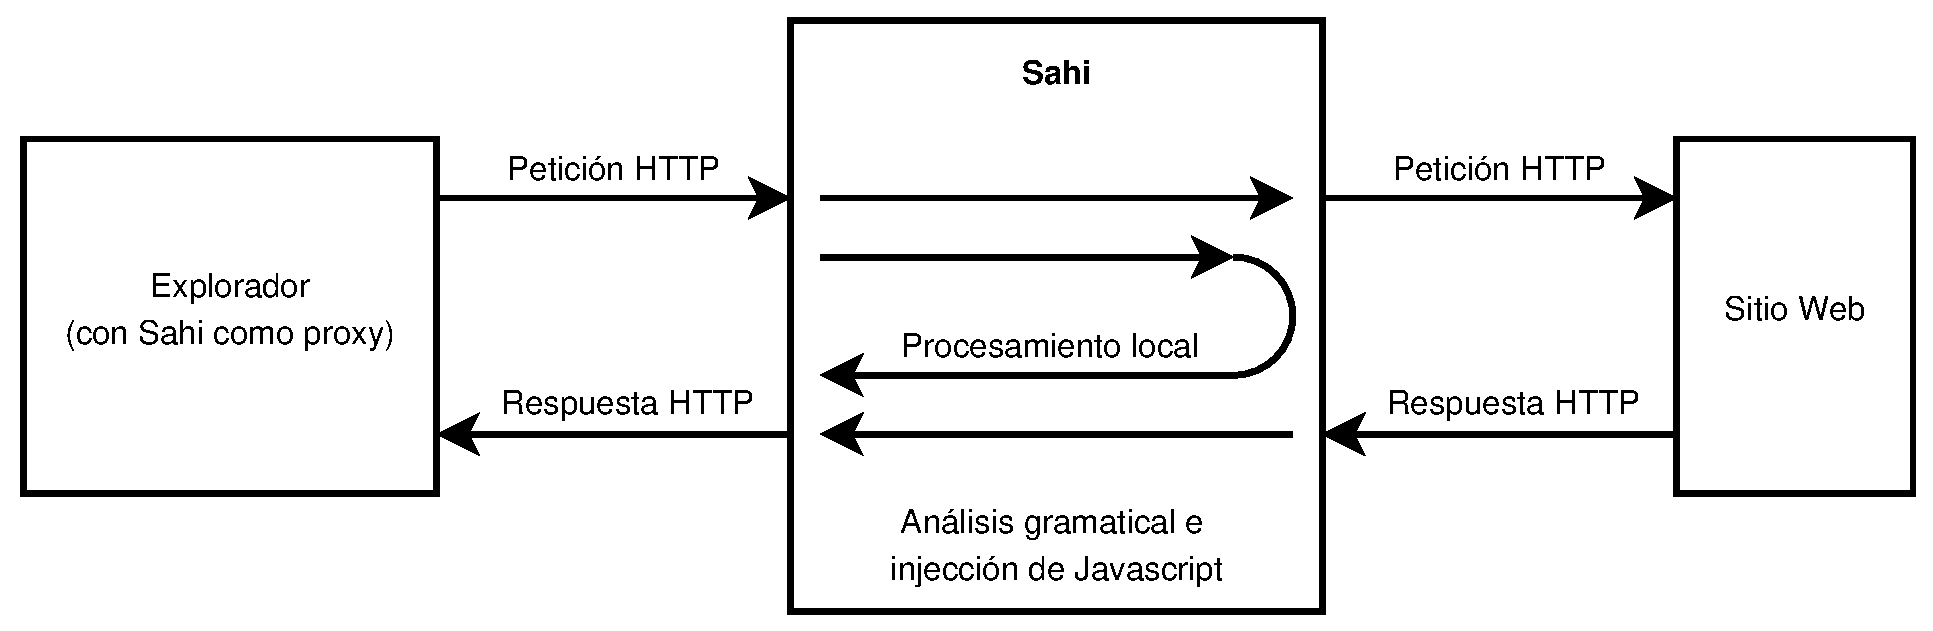
\includegraphics[width=\textwidth]{dia-sahi-arq}
\caption{Diagrama de flujo de Sahi\cite{SahiPro}.}
\label{fig:dia-sahi-arq}
\end{figure}

%\subsubsection{Java Data Base Controller}
%\subsubsection{Java IO}
%\subsubsection{Java Enterprise Edition}
%\subsection{Javascript}
%\subsection{Sahi}
%\subsection{iBatis}
%\subsection{Spring}
%\subsubsection{Spring MVC}
%\subsubsection{Spring JPA}
%\subsubsection{Spring Security}


\section{Implementación de base de datos}
El sistema AutoSA utiliza una base de datos relacional\footnote{Por confidencialidad no se hace mención específica del nombre y versión del sistema administrador de bases de datos.}(ver sección \ref{sec-bd-r}) para almacenar la información requerida en los casos de uso (ver sección \ref{sec:casos-uso}).\\
La implementación de la base de datos se ve reflejada en las rutinas con sentencias SQL (ver sección \ref{sec-bd-r}) donde se definen los objetos de la base de datos, tales rutinas se separan en dos grupos, las rutinas DDL y las rutinas DML.

\subsection{Rutinas de definición de datos}
Estas rutinas contienen las sentencias DDL (ver sección \ref{sec-bd-r}) para la creación de tablas, llaves primarias, llaves foráneas, índices y restricciones. En el código \ref{lst:sql-create-table} se muestra un ejemplo de la creación de una tabla.
\begin{lstlisting}[language=SQL, caption={Sentencia para crear una tabla.}, label={lst:sql-create-table}]
CREATE TABLE ordenes_is(
   id numeric(20,0) PRIMARY KEY NOT NULL,
   orden numeric(20,0) NOT NULL,
   estatus numeric(2,0) NOT NULL,
   id_sesion_insersion numeric(20,0) NOT NULL,
   id_sesion_estatus numeric(20,0) NOT NULL,
   estatus_sa numeric(2,0),
   estatus_sap numeric(2,0)
);
\end{lstlisting}

La generación de reportes que se menciona en el caso de uso \textbf{Generar reporte} (ver sección \ref{cu-generar-reporte}), utiliza una vista para la definición de la consulta de los datos del reporte (ver código \ref{lst:sql-create-view}, además se han implementado índices para agilizar tales consultas (ver código \ref{lst:sql-create-index}).

\begin{lstlisting}[language=SQL, caption={Sentencia para crear una vista.}, label={lst:sql-create-view}]
CREATE VIEW ordenes_contestadas AS
     SELECT *
       FROM ordenes_is
      WHERE id_sesion_estatus = :sesion
        AND estatus = 3
\end{lstlisting}

\begin{lstlisting}[language=SQL, caption={Sentencia para crear un índice.}, label={lst:sql-create-index}]
CREATE INDEX ordenes_contetadas_idx ON ordenes_is(id_sesion_estatus, estatus);
\end{lstlisting}

\subsection{Rutinas de modelado de datos}
Estas rutinas contienen la sentencias DML (ver sección \ref{sec-bd-r}) para insertar la información necesaria para la ejecución del sistema, como son, por ejemplo, los estados posibles de las órdenes de reposición (ver Figura \ref{fig:dia-estados-orden}), en el código \ref{lst:sql-insert} se muestra un ejemplo de la sentencia DML para insertar un registro.

\begin{lstlisting}[language=SQL, caption={Sentencia insertar un registro.}, label={lst:sql-insert}]
INSERT INTO cat_estatus_orden (id,nombre) VALUES (1,'NUEVA');
\end{lstlisting}

%================================================================================
%
%================================================================================

\section{Implementación de los componentes}

\subsection{Agente}
La implementación del componente Agente esta escrita en rutinas de Sahi (ver sección \ref{sec-sahi}), primero se mostrarán los puntos relevantes en la implementación de las rutinas de respuesta y envío de órdenes de reposición para después señalar como se realizar la ejecución mediante la herramienta gráfica de Sahi.

\subsubsection{Rutina para automatizar la respuesta de órdenes de reposición}\label{sec-aut-contestar}
La rutina para automatizar la respuesta de órdenes de reposición refleja el caso de uso  CU-CONTESTAR que se describe en la sección \ref{cu-contestar}, a continuación se muestran las secciones de código más relevantes de la rutina que realizan la ejecución del caso de uso citado así como los subsecuentes (ver diagrama en la Figura \ref{fig:dia-casos-uso}). A grandes rasgos, contestar las órdenes de reposición sigue los siguientes pasos:
\begin{enumerate}
	\item Ingresar al Sistema de Abastecimiento, en el código \ref{lst:sah-session} se muestra la rutina para iniciar sesión en el Sistema de Abastecimiento:
	\begin{enumerate}
		\item Las líneas 1 y 2 se llenan los campos de usuario y contraseña.
		\item La línea 3 se envía el formulario.
		\item La línea 4 redirige a la pantalla con el listado de órdenes de reposición.  
	\end{enumerate}
	\begin{lstlisting}[language=Javascript, caption={Inicio de sesión en el Sistema de Abastecimiento.}, label={lst:sah-session}]
_setValue(_textbox("Usuario[1]"), $user);
_setValue(_password("Contras[1]"), $pwd);
_click(_submit("Ingresar al Sistema"));
_click(_image("Normal[2]"));
	\end{lstlisting}

	\item Recolectar las órdenes de reposición listadas, el código \ref{lst:sah-save-news} muestra un resumen de la automatización para guardar el listado de ordenes de reposición (ver caso de uso en la sección \ref{cu-guardar-nueva}):
	\begin{enumerate}
		\item La línea 1 muestra la declaración del ciclo para recorrer el listado de órdenes de reposición.
		\item Las líneas 2 a 4 muestran como se extrae el valor de los datos de una orden de reposición.
		\item Las líneas 5 a 8 muestran la obtención de las URLs para contestar y enviar las órdenes de reposición.
		\item La línea 9 es el almacenamiento de la nueva orden de reposición. 
	\end{enumerate}
	\begin{lstlisting}[language=Javascript, caption={Guardar lista de órdenes de reposición.}, label={lst:sah-save-news}]
for(var $i = 1 + $errores; $i <= $rowCount; $i++){
	var $contrato = _getText(_table(1).rows[$i].cells[0]);
	var $solicitud = _getText(_table(1).rows[$i].cells[1]);
	var $numorden = _getText(_table(1).rows[$i].cells[2]);
	var $urlcon = "";
	_log(_table(1).rows[$i].cells[6].childNodes[0].href);
	_set($urlcon, _table(1).rows[$i].cells[6].childNodes[0].href);
	var $urlenv = $urlcon.replace("respoOra", "enviaOra");
	var $inserted = $persistence.insertOrden($contrato, $solicitud, $numorden, $expedicion, $almacen, $urlcon, $urlenv, $idSesion);
}
	\end{lstlisting}

	\item Contestar una a una cada orden de reposición, el código \ref{lst:sah-respond} muestra un resumen de la automatización para contestar una orden de reposición (ver caso de uso en la sección \ref{cu-responder-orden}):
	\begin{enumerate}
		\item Las líneas 1 y 2 muestran como se redirige al explorador a la URL para contestar la orden de reposición.
		\item  Las líneas 3 muestran como se estable un valor en el formulario para contestar la orden de reposición.
		\item La línea 4 realiza el envío del formulario.
		\item La línea 5 manda la actualización de la orden de reposición en la base de datos.
	\end{enumerate}
	\begin{lstlisting}[language=Javascript, caption={Responder orden de reposición.}, label={lst:sah-respond}]
var $url = $oimss.getUrlCon();
_navigateTo($url);
_setValue(_textbox("Lote"), "SL");
_click(_submit("Agregar Captura"));
$imss.updateCantidad($contrato, $numorden, $cantidad, $idSesion);
	\end{lstlisting}

	\item Enviar las órdenes de reposición contestadas, el código \ref{lst:sah-send} muestra un resumen de la automatización para envíar una órden de reposición (ver caso de uso en la sección \ref{cu-enviar-orden}):
	\begin{enumerate}
		\item Las líneas 1 y 2 muestran como se redirige al explorador a la URL para enviar la orden de reposición.
		\item La líneas 3 a 6 crea un mapa con los datos de la orden de reposición.
		\item La línea 7 actualiza la orden de reposición en la base de datos. 
	\end{enumerate}
	\begin{lstlisting}[language=Javascript, caption={Enviar orden de reposición.}, label={lst:sah-send}]
var $url = $entidad.getUrlEnv();
_navigateTo($url);
$mapa = new java.util.LinkedHashMap();
for(var $llave in $orden){
	$mapa.put($llave, $orden[$llave]);
}
$imss.updateOrdenImss($mapa, $idSesion);
	\end{lstlisting}
\end{enumerate}

\subsubsection{Rutina para automatizar la verificación de órdenes de reposición canceladas}
La rutina para automatizar la verificación de órdenes de reposición canceladas refleja el caso de uso  CU-VERIFICAR que se describe en la sección \ref{cu-verificar}, a continuación se muestran las secciones de código más relevantes de la rutina que realizan la ejecución del caso de uso citado así como los subsecuentes (ver diagrama en la Figura \ref{fig:dia-casos-uso}). Recordando que, a grandes rasgos, verificar las órdenes de reposición canceladas sigue los siguientes pasos:
\begin{enumerate}
	\item Ingresar al Sistema de Abastecimiento, el ingreso al sistema es idéntico a la rutina mostrada en la sección anterior (sección \ref{sec-aut-contestar}).

	\item Establecer los criterios de búsqueda, el código \ref{lst:sah-} muestra un resumen de la automatización para :
	\begin{enumerate}
		\item 
	\end{enumerate}
	\begin{lstlisting}[language=Javascript, caption={Responder orden de reposición.}, label={lst:sah-search}]
$dateLimits = $imss.getDateLimits('dd/MM/yyyy');
_setSelected(_select("OrdStt"), "Canceladas");
_setValue(_textbox("OrdFeD"), $dateLimits[0]);
_setValue(_textbox("OrdFeA"), $dateLimits[1]);
_click(_submit(0));
var $html = '';
_set($html, _table(5).innerHTML);
$estado = $imss.getCancelStatus();
$imss.setSaiStatus($html, $estado, $idSesion);
	\end{lstlisting}

	\item Extraer el listado de órdenes de reposición canceladas, el código \ref{lst:sah-} muestra un resumen de la automatización para :

	\item Actualizar el estado de las órdenes de reposición en la base de datos, el código \ref{lst:sah-} muestra un resumen de la automatización para :
\end{enumerate}










\subsubsection{Ejecución de las rutinas de automatización}
La ejecución de las rutinas de sahi corresponden a los casos de uso CU-CONTESTAAR y 
CU-VERIFICAR (ver secciones \ref{cu-contestar} y \ref{cu-verificar} respectivamente), en ambos casos la ejecucuión es  
dejando la ejecución al usuario por medio de la interfaz gráfica de Sahi:
\begin{itemize}
	\item Iniciar Sahi sobre el explorar de Internet (ver Figura \ref{fig:ss-sahi-dashboard})
	\begin{figure}[h]
	\centering
	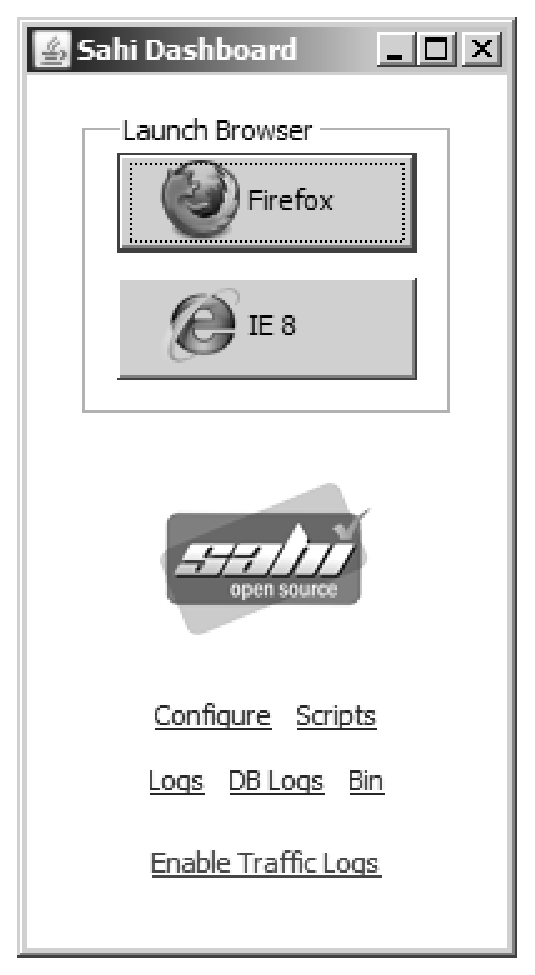
\includegraphics[scale=0.6]{ss-sahi-dashboard}
	\caption{Dashboard de Sahi.}
	\label{fig:ss-sahi-dashboard}
	\end{figure}

	\item Iniciar el controlador de Sahi y hacer los siguientes pasos (ver Figura \ref{fig:ss-sahi-controller}):
	\begin{enumerate}
		\item Seleccionar la rutina automatizada (contestar órdenes de reposición o verificación de órdenes de reposición)
		\item Ingresar la URL del Sistema de Abastecimiento
		\item Iniciar la ejecución.
	\end{enumerate}
	\begin{figure}[h]
	\centering
	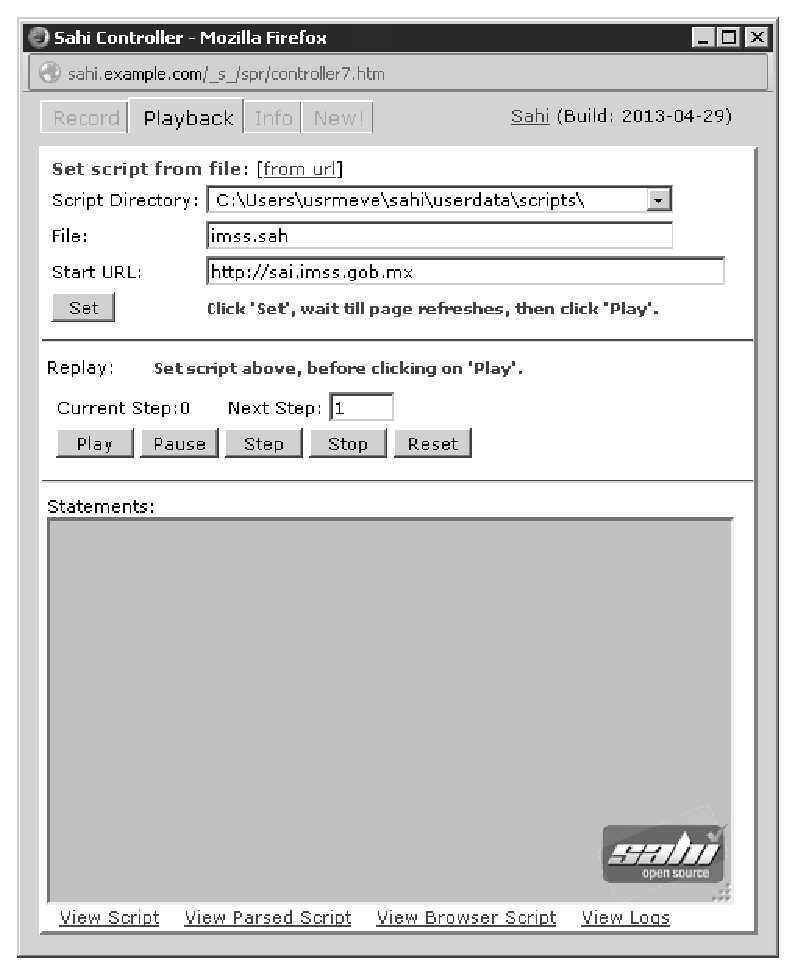
\includegraphics[scale=0.6]{ss-sahi-controller}
	\caption{Controlador de Sahi.}
	\label{fig:ss-sahi-controller}
	\end{figure}
\end{itemize}





\subsection{Lógica de Automatización}
	\paragraph{Respuesta\\}
		\textbf{guardar-orden-nueva}\\
		\textbf{obtener-datos-respuesta}\\
		\textbf{actualizar-orden-contestada}\\
		\textbf{guardar-orden-enviada}\\
		\textbf{obtener-acuse-envio}
	\paragraph{Verificación\\}
		\textbf{obtener-rango-fechas-verificar}\\
		\textbf{actualizar-estado-sa}

\subsection{Persistencia}
\subsubsection{Tecnologías utilizadas}
\textcolor{blue}{
\begin{enumerate}
	\item JDBC 			(Patrón factory)
	\item JPA			(Patrón proxy)
	\item SpringData	(Patrón proxy)
\end{enumerate}
}

\textcolor{blue}{
	Acá un diagrama que muestra las partes importantes del componente
}

\subsection{Sistema de archivos}
	\paragraph{Configuración\\}
		\textbf{obtener-propiedad}
	\paragraph{Almacenamiento\\}
		\textbf{guardar-archivo}


\subsection{Generador de reportes}

\textcolor{blue}{En el diseño debe agregarse un diagrama del funcionamiento de reportes: seleccionar templates... agregar patrones de diseño}\\
\subsection{Motor de plantillas}
\textcolor{blue}{aquí platico de volicity y como funciona el motor}\\
\textcolor{blue}{aquí va la configuración}\\
\textcolor{blue}{tipos de reporte}

	\paragraph{Acuse\\}
		\textbf{generar-acuse-envio}
	\paragraph{Generación\\}
 		\textbf{generar-reporte-ordenes}


\subsection{Portal Web}
\textcolor{blue}{Las secciones de esta parte serán presentadas por capas desde datos hasta la vista}\\
\textcolor{blue}{Presentar el patron MVC}\\
\subsection{Acceso}
\textcolor{blue}{Spring security}\\
\textcolor{blue}{Cifrado de contraseña}\\
\subsection{Generación de reportes}
\subsection{Búsqueda}

\subsection{Administración de catálogos}

\subsection{Visualización de órden de reposición}

\subsection{Edición de órden de reposición}









%\section{Implmenetación de genración de reportes}

%\section{Implementación de automatización para SA}
%\subsection{Bibliotecas para las rutinas de automatización}
%\subsection{Rutinas de automatización}




